%
% LaTeX report template 
%

\documentclass[11pt, a4paper]{article}
\usepackage{graphicx}
\usepackage{amsmath}
\usepackage{listings}
\usepackage{url}
\usepackage{float}
\usepackage{xcolor}

\definecolor{codegreen}{rgb}{0,0.6,0}
\definecolor{codegray}{rgb}{0.5,0.5,0.5}
\definecolor{codepurple}{rgb}{0.58,0,0.82}
\definecolor{backcolour}{rgb}{0.95,0.95,0.92}

\lstdefinestyle{mystyle}{
    backgroundcolor=\color{backcolour},   
    commentstyle=\color{codegreen},
    keywordstyle=\color{magenta},
    numberstyle=\tiny\color{codegray},
    stringstyle=\color{codepurple},
    basicstyle=\ttfamily\footnotesize,
    breakatwhitespace=false,         
    breaklines=true,                 
    captionpos=b,                    
    keepspaces=true,                 
    numbers=left,                    
    numbersep=5pt,                  
    showspaces=false,                
    showstringspaces=false,
    showtabs=false,                  
    tabsize=2
}

\lstset{style=mystyle}

\title{EE2703: Applied Programming Lab \\ End Semester Examination} % Title

\author{Ishaan Agarwal \\ EE20B046} % Author name

\date{\today} % Date for the report
\begin{document}		
		
\maketitle % Insert the title, author and date

\section{Introduction}
A long wire carries a current I(z) in a dipole antenna given by:
\[I = Im\sin(k(l - |z|))\]
We want to use this to compute the radiated field. The problem is to determine if this is a good assumption. 

\section{Questions}
The parameters of the dipole antenna are defined as follows:\\$l = 0.5$ m (quarter wavelength),\\ $c = 2.9979 \cdot 10^8$ m/sec (speed of light),\\ $\mu_0 = 4 \pi \cdot 10^-7$ (permeability of free space),\\ $N = 4$ (Number of sections in each half of the antenna),\\
$I_m = 1$ A (current injected into the antenna),\\ $a = 0.01$ m (radius of wire),\\ $\lambda = l * 4$ m (wavelength),\\
$f = c / \lambda$ Hz (frequency),\\ $k = 2 \pi / \lambda$ $meter^{-1}$(wave number),\\ $dz = l / N$ (spacing of current samples).

We add this to our code file as follows:\\
\begin{lstlisting}[language = Python]
#defining the constants

#independent parameters
l = 0.5 #quarter wavelength
c = 2.9979e8 #speed of light
mu0 = 4*np.pi*1e-7 #permeability of free space
N = 4 #Number of sections in each half section of the antenna
Im = 1 #current injected into the antenna
a = 0.01 #radius of the wire

#dependent parameters
lamda = l*4 #wavelength 
f = c/lamda #frequency
k = 2*np.pi/lamda #wave number
dz = l/N #spacing of the elements


\end{lstlisting}



\subsection{Question 1: Creating the vectors}
We divide the wire into pieces of length $dz$. We make four arrays, $z, u, I$ and $J$ where, z is the location of all the currents, u is the location of the unknown currents only, I are the current values at the positions given by z, and J are the current values at the positions given by u. \\Since, the end currents are known to be $0$ and the current at the centre is known to be $Im$, we have, dimensions of $u, J = 2*N-2$ and dimensions of $z, I = 2*N+1$. All of this is done using the following piece of code.\\ 

\begin{lstlisting}[language = Python]
#Question 1
z = np.zeros(2*N+1)
z = np.linspace(-l, l, 2 * N + 1) #creating the array of z and dropping certain values to obtain the array of u
#drop first and last element and middle element of u (known values)
u = np.delete(z, [0, N, -1])

#constructing current vectors (theoretical)
I = Im * np.sin((2 * np.pi / lamda) * (l - abs(z)))  # current vector
I[N] = Im #current injected into the middle element
I[0] = 0 #boundary condition
I[-1] = 0 #boundary condition
#form J by deleting first, last and middle element of I
J = np.delete(I, [0, N, -1])
\end{lstlisting}

\subsection{Question 2: M Matrix}
Now, our aim is to find each unknown current. From Ampere's Law, we get for $H_\phi(z, r = a)$:

\begin{equation*}
    2\pi a H_\phi(z_i) = I_i
\end{equation*}

In matrix form:
\begin{equation*}
    \begin{pmatrix}
        H_\phi[z_1] \\ \dots \\ H_\phi[z_{N-1}] \\ H_\phi[z_{N+1}] \\ \dots \\ H_\phi[z_{2N-1}]
    \end{pmatrix}
    = \frac{1}{2\pi a} I_{2N-2}
    \begin{pmatrix}
        J_1 \\ \dots \\ J_{N-1} \\ J_{N+1} \\ \dots \\ J_{2N-1}
    \end{pmatrix}
    = M * J
\end{equation*}
Where $I_{2N-2}$ represents the Identity matrix of order $2N-2$\\ 
So, we write a function to compute M matrix, given by:\\

\begin{lstlisting}[language = Python]
#Question 2
#creating M matrix which is 1/(2*pi*a) * Identity matrix (dimension = 2*N-2)
def compute_M(N, a):
    M = np.identity(2*N-2)*(1/(2*np.pi*a))
    return M
M = compute_M(N, a)

\end{lstlisting}

\subsection{Question 3: $R_z, R_u, P$ and $P_B$}

\subsubsection*{Vector potential equation}

\begin{equation*}
    \vec{A}(r, z) = \frac{\mu_0}{4\pi} \int \frac{I(z')\hat{z}e^{-jkR}dz'}{R}
\end{equation*}

This is further reduced to a sum:

\begin{equation*}
    A_{z, i} = \sum_j I_j \frac{\mu_0}{4\pi} \frac{e^{-jkR_{ij}}}{R_{ij}} dz'_j
\end{equation*}

\begin{equation*}
    A_{z, i} = \sum_j P_{ij} I_j + P_B I_N
\end{equation*}

In this equation, $P_ij$ accounts for all current elements except $I_N$, whereas $P_B$ is used to account for the contribution to the vector potential due to  the current $I_N$ and is given by 

\begin{equation*}
    P_B = \frac{\mu_0}{4\pi}  \frac{e^{-jkR_{iN}}}{R_{iN}}dz'_j
\end{equation*}

The code for this part is as follows:\\

\begin{lstlisting}[language = Python]

#Question 3
#computing Rz and Ru
#Rz computes distances including distances to known currents whereas Ru computes distances for only unknown currents
def compute_Rz(z, z_dash):
    return np.sqrt((z-z_dash)**2 + a**2)
def compute_Ru(u, u_dash):
    return np.sqrt((u-u_dash)**2 + a**2)

Rz = compute_Rz(u, z.reshape(-1,1))
Ru = compute_Ru(u, u.reshape(-1,1))

\end{lstlisting}

We then compute $P$ and $P_B$ as follows:\\

\begin{lstlisting}[language = Python]

#computing P and Pb
def compute_P(Ru):
    return (mu0/(4*np.pi)) * np.exp(-1j*k*Ru) * (1/Ru) * dz
def compute_Pb(RiN):
    return (mu0/(4*np.pi)) * np.exp(-1j*k*RiN) * (1/RiN) * dz

P = compute_P(Ru)
Pb = compute_Pb(Rz[N,:])


\end{lstlisting}

\subsection{Question 4: $H_\phi(r,z)$, $Q_{ij}$ and $Q_B$}
From our knowledge of electromagnetics, simplifying the expressions, we get:
\begin{align*}
    H_\phi(r, z_i) & = -\sum_{j} \frac{dz^{'}_j}{4\pi}(\frac{-jk}{R_{ij}}-\frac{1}{R^2_{ij}})\exp(-jkR_{ij})\frac{rI_j}{R_{ij}}                                \\
                   & = -\sum_{j}P_{ij}\frac{r}{\mu0}(\frac{-jk}{R_{ij}}-\frac{1}{R^2_{ij}})I_j + P_{B}\frac{r}{\mu0}(\frac{-jk}{R_{iN}}-\frac{1}{R^2_{iN}})I_m \\
                   & = \sum_{j}Q^{'}_{ij}I_j                                                                                                                   \\
H_\phi(r, z_i)                   & = \sum_{j}Q_{ij}I_{j} + Q_{Bi}Im
\end{align*}

To compute $Q_{ij}$ and $Q_B$, the following code is used:\\

\begin{lstlisting}[language = Python]
#Question 4
#computing Qij and Qb
def compute_Qij(Ru, P):
    return -P * (a / mu0) * (complex(0, -k) / Ru - 1 / Ru**2)
def compute_QB(Pb, RiN):
    return -Pb * a / mu0 * ((-1j * k) / RiN - 1 / (RiN**2))

Qij = compute_Qij(Ru, P)
Qb = compute_QB(Pb, Rz[N,:])
Qb = Qb.reshape(-1,1)
\end{lstlisting}

\subsection{Question 5: Final Equation and Plotting the results}
We have derived $H_\phi$ in two ways, equating both of them, we get:
\begin{align*}
    MJ                & = QJ + Q_B I_m         \\
     (M - Q)J & = Q_B I_m              \\
    \implies J        & = (M - Q)^{-1} Q_B I_m
\end{align*}
thus, implementing this in python to find $J$, we write: \\
\begin{lstlisting}[language = Python]
#Question 5
#finding J_calculated and I_calculated
J_calculated = (np.linalg.inv(M-Qij).dot(Qb*Im)).T[0] #obtained was an array of array, thus taking the first element of the array
I_calculated = np.concatenate(([0], J_calculated[:N-1], [Im], J_calculated[N-1:], [0])) 


\end{lstlisting}

We now plot the calculated value of the current vector against the value of the current vector which was obtained assuming sinusoidal variation. This is done as follows: \\

\begin{lstlisting}[language = Python]
#plotting I and I_calculated on the same graph
plt.plot(z, I, label = 'I(assuming sine wave)')
plt.plot(z, I_calculated, label = 'I_calculated')
plt.title('Calculated current vs Assumed current Plot')
plt.grid()
plt.xlabel('z')
plt.ylabel('I')
plt.legend(loc = 'upper right')
plt.show()

\end{lstlisting}

The following plot is obtained:

\begin{figure}[H]
     \centering
     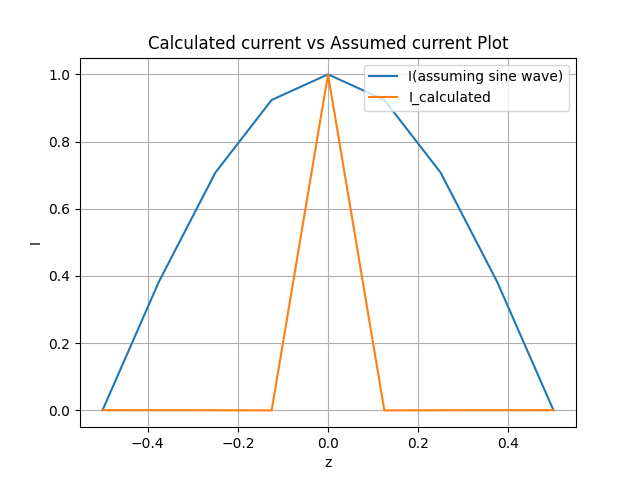
\includegraphics[scale=0.8]{Figure_1.png}
\end{figure}

Repeating the exercise for $N=100$, the following plot is obtained:

\begin{figure}[H]
     \centering
     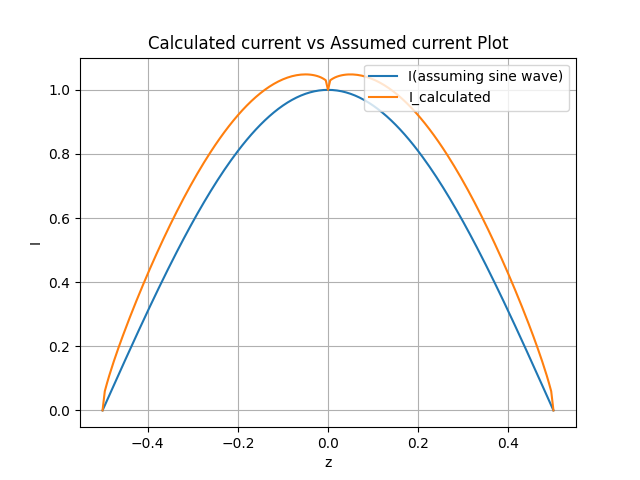
\includegraphics[scale=0.8]{Figure_2.png}
\end{figure}

At the end, we compile and print out all our obtained results using the following piece of code:\\

\begin{lstlisting}[language = Python]
#printing all values for N=4
print('\n')
print('N = 4')
print('\n')
print('z = ', z.round(2))
print('\n')
print('u = ', u.round(2))
print('\n')
print('M = ', M.round(2))
print('\n')
print('Rz = ', Rz.round(2))
print('\n')
print('Ru = ', Ru.round(2))
print('\n')
print('RiN = ', Rz[N,:].round(2))
print('\n')
print('P = ', (P*1e8).round(2))
print('\n')
print('Pb = ', (Pb*1e8).round(2))
print('\n')
print('Qij = ', Qij.round(2))
print('\n')
print('Qb = ', Qb.round(2))
print('\n')
print('J_calculated = ', J_calculated.round(6))
print('\n')
print('I_calculated = ', I_calculated.round(6))
print('\n')


\end{lstlisting}

The following results are obtained:

\begin{figure}[H]
     \centering
     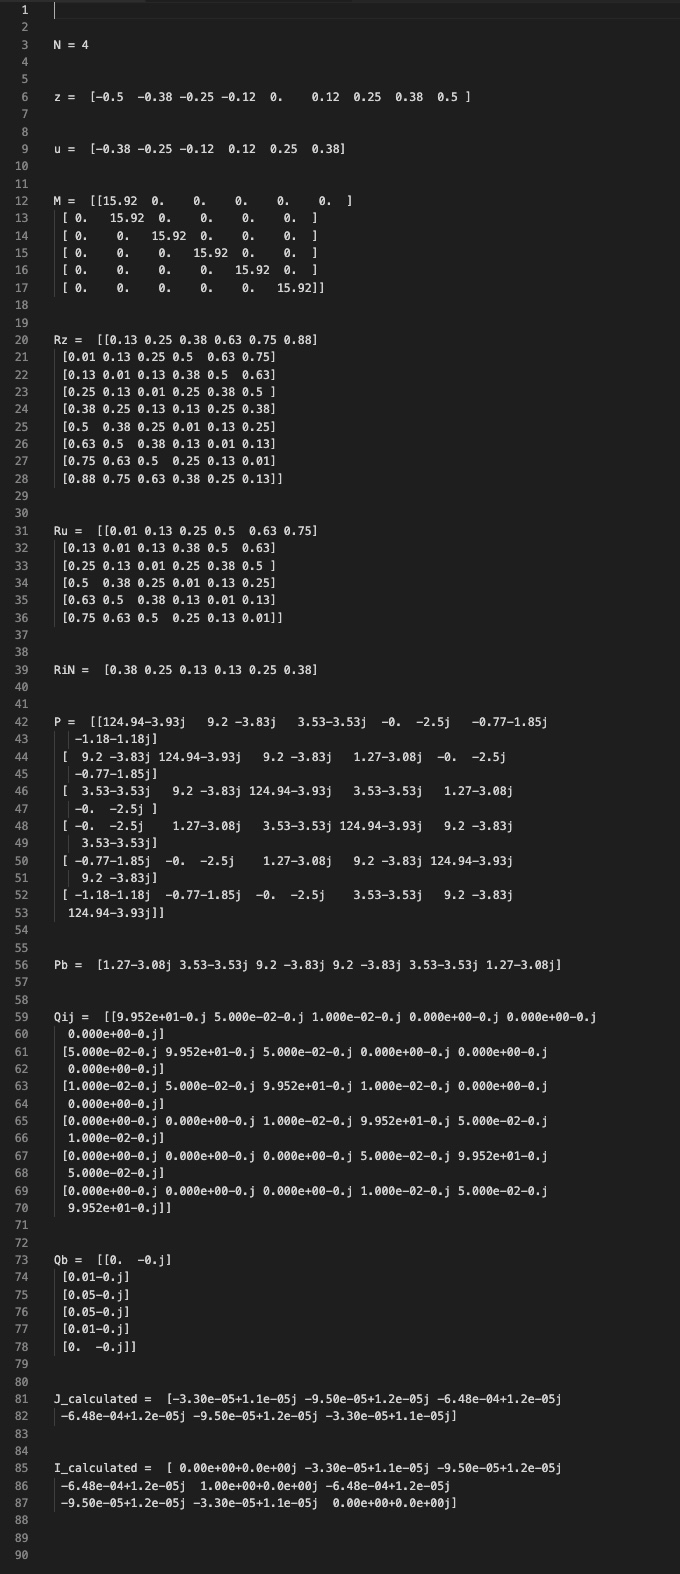
\includegraphics[scale=0.9]{Figure_3.png}
\end{figure}






\section{Conclusion}
Integration (where $dz$ is infinitesimal) was approximated as summation with finite $dz$ and as seen from the obtained plots, our assumption is significantly reasonable, and thus we can say that the current distribution is approximately sinusoidal. This is also highlighted by the fact that as the value of N rose from $N=4$ to $N=100$, we got a more accurate solution.\\ We have learnt how to deal with matrix equations and solving them, we have also learnt how to avoid using loops and using vectorised code instead. We have also plotted and visualised our results.


\end{document}



 